%\cleardoublepage
\mbox{}

\lstset{
language=Python,
basicstyle=\small\sffamily,
numbers=left,
numberstyle=\tiny,
frame=tb,
columns=fullflexible,
showstringspaces=false
}

\chapter{Tecnología OpenVINO}
\label{ch:chapter3}

OpenVINO es un conjunto de herramientas multiplataforma desarrolladas por Intel, que facilita la transición entre los entornos de entrenamiento y producción de nuestro modelo de aprendizaje profundo.
A pesar de estar desarrollada por una empresa comercial como Intel, pertenece al conjunto de aplicaciones de código abierto, de modo que se puede visualizar su código fuente, reportar fallos e incluso realizar aportaciones.


El cometido principal de esta aplicación es la optimización del tiempo de inferencia de un modelo de Deep Learning previamente entrenado.
Para ello, OpenVINO dispone de su propio formato de definición de modelos.
Estos archivos son los que procesa su propia red de inferencia multiplataforma, ya que se encuentra preparada para poder trabajar de manera concurrente, aprovechando así toda la potencia de los procesadores o GPU actuales \cite{gpu_solution}.

En la siguiente Figura~\ref{fig:Arquitectura de optimización de modelos con OpenVINO} se puede observar el flujo de trabajo que se ha seguido en este trabajo, haciendo uso de la herramienta OpenVINO.
En primer lugar, optimizaremos la topología de nuestro modelo y obtendremos una nueva representación del mismo, pero esta vez, con el formato necesario para ser procesado por la red de inferencia de alto rendimiento de OpenVINO.
Finalmente, nuestra red de inferencia será la que realice el trabajo de clasificación en el entorno de producción de nuestra aplicación.

Podemos visualizar el código de la aplicación en su repositorio oficial de GitHub\footnote{\url{https://github.com/openvinotoolkit/openvino}}.


\begin{figure}
    \centering
    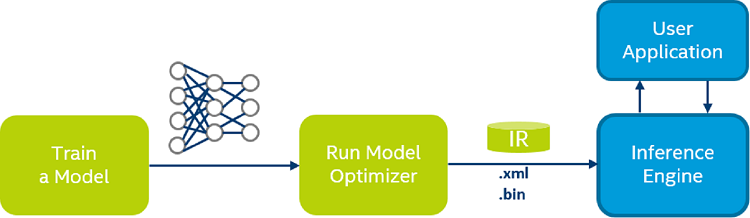
\includegraphics[width=0.8\textwidth]{images/chapter3/openvino_workflow.png}
    \caption{Arquitectura de optimización de modelos con OpenVINO.}
    \label{fig:Arquitectura de optimización de modelos con OpenVINO}
\end{figure}


\section{Herramientas que lo componen}\label{sec:herramientas-que-lo-componen}
Esta tecnología desarrollada por Intel tiene por objetivo principal la optimización de modelos de redes neuronales convolucionales para potenciar su velocidad de inferencia.
OpenVINO es capaz de soportar distintos hardwares (FPGA, Intel Movidius, procesamiento por GPU\@) y también varios sistemas operativos (Mac Os, Linux o Windows).

Las características principales de esta aplicación se resumen en dos puntos:

\begin{itemize}
    \item \textbf{Optimizador de modelos de \texit{Deep Learning}}: Aplicación de interfaz de línea de comando, la cual usa como base modelos de frameworks populares como Caffe, TensorFlow, MXNet, Kaldi y ONNX para convertirlos a un modelo optimizado de OpenVINO.
    \item \textbf{Interfaz de inferencia de modelos de \texit{Deep Learning}}: API de alto rendimiento multiplataforma para realizar la inferencia de manera rápida y eficiente sobre dispositivos de Intel.
\end{itemize}

\subsection{Optimizador de modelos de \texit{Deep Learning}}\label{subsec:optimizador-de-modelos-de-deep-learning}
Para poder realizar la optimización de nuestro modelo de \texit{Deep Learning} previamente entrenado, se necesita el binario que contiene la topología de la red del modelo.
Una vez el optimizador de OpenVINO procesa nuestro modelo procede a realizar una conversión de cada capa interna de la red a una nueva capa.
Esta nueva capa, ya convertida al formato de OpenVINO, conserva los pesos de la red anterior,
sin embargo, está preparada para que la aplicación de inferencia de OpenVINO pueda leerla correctamente.

Esta herramienta proporciona de manera genérica distintos scripts para realizar esta conversión.
Se incluyen diferentes ficheros de código fuente para los frameworks de \texit{Deep Learning} más actuales, codificados en Python y totalmente modificables, aunque en principio no es necesario porque ya vienen preparados para funcionar.

\subsection{Interfaz de inferencia de modelos de \texit{Deep Learning}}
\label{subsec:interfaz-de-infernecia-de-modelos-de-deep-learning}
Con nuestro modelo y su topología convertida a un formato válido de OpenVINO, ya tenemos todo lo necesario para poder realizar clasificaciones con su interfaz de inferencia\@.
La optimización de inferencia se produce en este punto, donde cada capa de nuestro modelo original es procesada por la aplicación en un lenguaje de bajo nivel, preparado para realizar operaciones vectoriales bajo total control del programador.
El lenguaje empleado para la codificación de la aplicación es C++ pese a que el programa pueda ser utilizado también en Python.
Esto se debe al uso de su API, que traduce las peticiones realizadas en Python al core de la interfaz, que es C++ puro.

Todas las capas usadas en este proyecto son compatibles de manera directa con las predefinidas por la interfaz de inferencia, incluidas en la versión de OpenVINO 2020.1.023.
OpenVINO nos da la posibilidad de añadir capas personalizadas, con el inconveniente de que deben ser programadas por el usuario de manera explícita en C++ para hacerlas compatibles con el resto de la aplicación, y, por supuesto, mantener estas nuevas capas a lo largo de las distintas actualizaciones y posibles cambios que pueda sufrir la aplicación.


\section{Conversión del modelo a la plataforma OpenVINO}\label{sec:conversión-del-modelo-a-la-plataforma-OpenVINO}
Para realizar la conversión, en primer lugar es necesaria la exportación del original de TensorFlow a un formato compatible con la red de optimización de modelos de OpenVINO\@.

La serialización por defecto de un modelo de TensorFlow puede incluir de manera independiente:

\begin{itemize}
    \item Un punto de control TensorFlow que contiene los pesos del modelo.
    \item Un prototipo `SavedModel' que contiene la topología de la red del modelo de TensorFlow.
\end{itemize}

Los métodos exactos para la serialización del modelo varían según la versión de TensorFlow, en este caso 1.15.2. La metodología de conversión exacta utilizada
para este proyecto se puede encontrar en el repositorio de código fuente en GitHub\footnote{\url{https://github.com/A-Ortiz-L/multispectral-imaging-cnn-final-degree-work/blob/master/src/entity/keras\_model.py}}.
Este modelo de OpenVINO va a servir tanto de punto de partida para su optimización como para su uso directo en el servicio personalizado de TensorFlow, con el objetivo de desplegar modelos en producción.

Una vez exportado el modelo de \texit{Deep Learning} al formato estándar de TensorFlow, tendremos a nuestra disposición los ficheros necesarios para proceder a su transformación al formato de OpenVINO.
Para realizar esta operación se hace uso de la herramienta de optimización de modelos, en concreto, con el script específico de TensorFlow, cuyo nombre
es \texttt{mo\_tf.py}. Este código fuente es ejecutado en la línea de comandos del sistema operativo correspondiente con los siguientes parámetros:


\begin{lstlisting}[caption=Comando de terminal para convertir un modelo TensorFlow a uno de OpenVINO.,
  label=a_label]
    mo_tf.py --input_model model.pb --input_model_is_text -b 1
\end{lstlisting}

El comando usado epecifica con el flag \texttt{--input\_model\_is\_text} que nuestro fichero no está codificado en binario, por lo que es texto plano.
Esta opción es totalmente configurable y depende del proceso de exportación.
Se ha encontrado útil la opción de exportación a texto plano ya que de esta manera
se puede observar la arquitectura de la red y los pesos pertenecientes a cada capa.

Configuramos también el \textit{flag} -b, esta opción determina el valor de reemplazo cuando se reciben valores negativos. Seleccionamos como valor uno porque en las entradas de nuestra red neuronal pueden propagarse valores
negativos, los cuales no son válidos para su procesamiento en OpenVINO\@.

\section{Inferencias. TensorFlow vs OpenVINO}\label{sec:inferencias.-Tensorflow-vs-OpenVINO}
Como se ha mencionado anteriormente, Tensorflow posee su propio sistema de inferencia preparado para su uso productivo en un entorno real. Este sistema se llama TensorFlow serving, que incorpora un servidor codificado mediante el patrón diseño API REST\footnote{\url{https://stackoverflow.blog/2020/03/02/best-practices-for-rest-api-design/}}, de modo que las peticiones de inferencia se realizan al servidor por medio del protocolo de transmisión de datos HTTP.
La aplicación de TensorFlow está diseñada para el escalado tanto en el número de modelos para los que puede recibir inferencias y sus versiones, como para la escalabilidad en capacidad de cálculo.
El escalado de cálculo está preparado para funcionar en una arquitectura clúster, en este caso de contenedores como es Kubernetes\footnote{\url{https://kubernetes.io/es/docs/concepts/overview/what-is-kubernetes/}}, por lo que el servidor puede ser encapsulado en su totalidad en un contenedor de Docker. Para este proyecto se ha trabajado con una versión encapsulada de Docker, pero no con la extensibilidad del escalado con Kubernetes~\cite{kubernetes}.
La unidad de cálculo principal del sistema de inferencia también se puede configurar, lo que permite el uso tanto de CPU como de GPU.
Por esa razón, en caso de que se decida emplear esta tecnología junto con una GPU, es necesario configurar de manera explicita el entorno.

En la Figura~\ref{fig:Arquitectura de TensorFlow serving} podemos observar el diseño de la arquitectura de la aplicación. Una de las ventajas frente a usar el sistema de inferencias clásico de TensorFlow es que la aplicación está preparada y optimizada para recibir tanto peticiones en streaming como en batch. Adicionalmente, reducimos el tamaño de las librerías a instalar al mínimo necesario para realizar las inferencias y configurar el servidor. Esta solución es más ligera y portable, evitando así instalar todo el sistema de construcción de algoritmos y demás artefactos que incorpora la librería de TensorFlow para programar redes neuronales.

\begin{figure}[h]
    \centering
    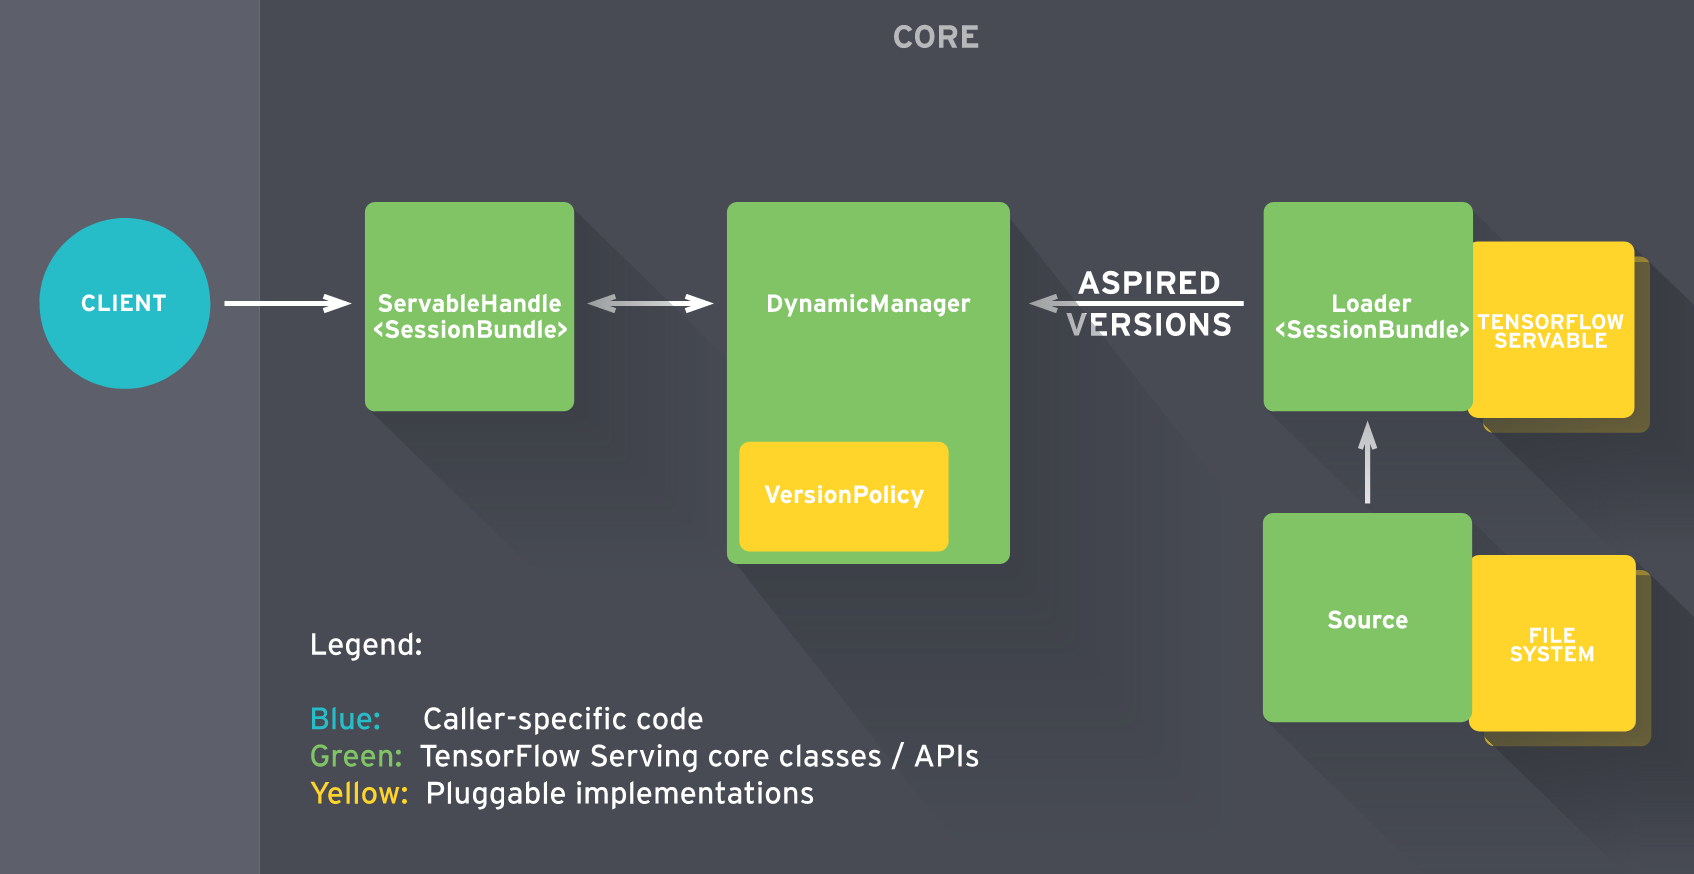
\includegraphics[width=1.0\textwidth]{images/chapter3/tf_serving_architecture.png}
    \caption{Arquitectura de TensorFlow serving.}
    \label{fig:Arquitectura de TensorFlow serving}
\end{figure}

La inicialización del servidor de inferencia y los métodos necesarios para realizar la petición aparecen en el Código~\ref{example2}. En su inicialización arrancamos el servidor REST, que funcionará de forma transparente para el usuario de nuestra aplicación, ya que se ejecuta en la red local de nuestro contenedor Docker.

\begin{lstlisting}[caption=Código Python para la red de inferencia de TensorFlow.,
      label=b_label,
      language=Python,label={example2}]
class TensorflowNetwork:
    def __init__(self):
        self.model_uri = 'http://localhost:8501/v1/models/model:predict'
        self.init_tensorflow_serve()

    @staticmethod
    def shape_image(file_route):
        img_array = cv2.imread(file_route, cv2.IMREAD_GRAYSCALE)
        new_array = cv2.resize(img_array, (128, 128))
        img = new_array.reshape(-1, 128, 128, 1) / 255.0
        img = np.float32(img).tolist()
        return img

    def process_image(self, file_route) -> Tuple[bool, float]:
        image = self.shape_image(file_route)
        start = time.time()
        predict = self.network_request(image)
        return predict, (time.time() - start)

    def network_request(self, image) -> bool:
        headers = {"content-type": "application/json"}
        data = json.dumps({"signature_name": "serving_default", "instances": image})
        res = requests.post(self.model_uri, data=data,
                            headers=headers)
        predictions = json.loads(res.text)['predictions']
        predict = True if predictions[0][0] >= 0.5 else False
        return predict

    @staticmethod
    def init_tensorflow_serve():
        os.system('tensorflow_model_server '
                  '--rest_api_port=8501 --model_name=model '
                  '--model_base_path=/app/model &')
\end{lstlisting}

Por otro lado, OpenVINO también incorpora en su conjunto de herramientas un sistema de inferencia optimizado.
Al igual que el sistema de inferencia de TensorFlow, OpenVINO también puede configurar tanto un procesador como una tarjeta gráfica para realizar sus cálculos.
La aplicación de inferencia de OpenVINO usada en este trabajo se codifica de manera íntegra haciendo uso del lenguaje de programación Python. Podemos observar esta implementación en el Código~\ref{example}.

\begin{lstlisting}[caption=Código Python para la red de inferencia de OpenVINO.,
    label=a_label,
    language=Python,label={example}]
    class OpenVinoNetwork:
    def __init__(self):
        self.plugin = IEPlugin(device='CPU')
        self.net = IENetwork(model=f'{pickle_dir}model.xml',
                             weights=f'{pickle_dir}model.bin')
        self.exec_net = self.plugin.load(network=self.net)

        self.input_blob = next(iter(self.net.inputs))
        self.out_blob = next(iter(self.net.outputs))
        self.net.batch_size = 1
        self.image_shape = 128

    def process_image(self, image_path) -> Tuple[bool, float]:
        image = self.shape_image(image_path)
        start = time.time()
        res = self.network_request(image)
        return res, time.time() - start

    def shape_image(self, file_route):
        image = cv2.imread(file_route, cv2.IMREAD_GRAYSCALE)
        image = cv2.resize(image, (self.image_shape, self.image_shape))
        image = image.reshape(self.image_shape, self.image_shape) / 255.0
        return image

    def network_request(self, image) -> bool:
        res = self.exec_net.infer(inputs={self.input_blob: image})
        res = res[self.out_blob]
        res = False if res < 0.5 else True
        return res
\end{lstlisting}

En su inicialización se lee el fichero ya optimizado del modelo de \texit{Deep Learning}, también se inicia la clase
perteneciente a la API de inferencia de OpenVINO que se encarga de realizar las inferencias.
Se configuran métodos específicos para transformar la imagen a las dimensiones correspondientes y para hacer la petición a la red.
La potencia de este modelo reside en la optimización que realiza la red en un lenguaje de bajo nivel, centrándose así en reducir los tiempos de inferencia.

Ambas soluciones implementan tecnologías de contenedores mantenidos de manera oficial por los fabricantes\footnote{\url{https://hub.docker.com/u/openvino}}\textsuperscript{,}\footnote{\url{https://hub.docker.com/r/tensorflow/tensorflow/}}, por lo que el uso de Docker es la mejor opción para transportar
nuestras redes de inferencia a cualquier sistema o dispositivo hardware.
Como punto distintivo, OpenVINO implementa soluciones de fábrica para FPGA e Intel Movidius. Las opciones de portabilidad son más amplias en esta tecnología, aunque no se descarta el uso de TensorFlow en estas plataformas, ya que su código fuente es accesible para todo el mundo y puede ser modificado.
De manera adicional y como paso natural, las dos herramientas se han preparado para ser incluidas en un clúster de contenedores\footnote{\url{https://github.com/openvinotoolkit/model_server}}\textsuperscript{,}\footnote{\url{https://www.tensorflow.org/tfx/serving/serving_kubernetes}}.



